\documentclass{article}
\usepackage{ProfLycee}
\useproflyclib{ecritures}
\usepackage{tikz}
\begin{document}

  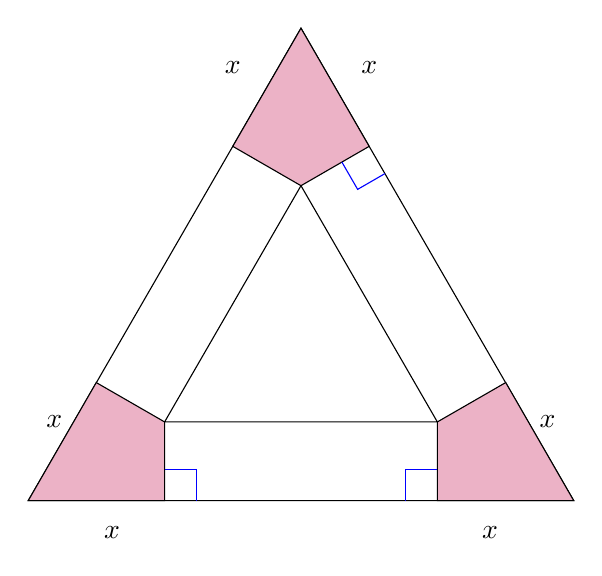
\begin{tikzpicture}[scale=2]
    % Define coordinates for the outer triangle
    \coordinate (A) at (0,2);
    \coordinate (B) at (-1.732,-1);
    \coordinate (C) at (1.732,-1);
  
    % Draw the outer triangle
    \draw (A) -- (B) -- (C) -- cycle;
  
    % Define coordinates for the inner triangle
    \coordinate (A1) at (0,1);
    \coordinate (B1) at (-0.866,-0.5);
    \coordinate (C1) at (0.866,-0.5);
  
    % Draw the inner triangle
    \draw (A1) -- (B1) -- (C1) -- cycle;
  
    % Define coordinates for the corner triangles
    \coordinate (A2) at (-0.433,1.25);
    \coordinate (A3) at (0.433,1.25);
    \coordinate (B2) at (-1.3,-0.25);
    \coordinate (B3) at (-0.866,-1);
    \coordinate (C2) at (1.3,-0.25);
    \coordinate (C3) at (0.866,-1);
  
    % Draw the corner triangles and fill them
    \filldraw[fill=purple!30] (A) -- (A2) -- (A1) -- (A3) -- cycle;
    \filldraw[fill=purple!30] (B) -- (B2) -- (B1) -- (B3) -- cycle;
    \filldraw[fill=purple!30] (C) -- (C2) -- (C1) -- (C3) -- cycle;
  
   
    % Mark right angles
    \draw[blue] (A3)++(0.1,-0.1732) -- ++(-0.1732,-0.1) -- ++(-0.1,0.1732);
    \draw[blue] (B3)++(0.2,0) -- ++(0,0.2) -- ++(-0.2,0);
    \draw[blue] (C3)++(-0.2,0) -- ++(0,0.2) -- ++(0.2,0);
  
    % Add x labels
    \node at (-0.433,1.75) {$x$};
    \node at (0.433,1.75) {$x$};
    \node at (-1.566,-0.5) {$x$};
    \node at (-1.2,-1.2) {$x$};
    \node at (1.2,-1.2) {$x$};
    \node at (1.566,-0.5) {$x$};
  
  \end{tikzpicture}
  



Correction;:

Calculons le volume de la boîte en fonction de $x$.

On note $\ell$ la longueur d'un côté de la boîte. On a alors $\ell = 60-2x$.

Il reste à calculer l'aire du fond de la boîte, c'est-à-dire l'aire du triangle équilatéral de côté $\ell$.




\end{document}